\clearpage
\subsection{Local Variable} % (fold)
\label{sub:local_variable}

Variables can be declared at a number of different places in your code. Variables that are declared within Procedures are called \textbf{Local Variables}. Most of the variables in your code will be Local Variables.

\begin{figure}[h]
   \centering
   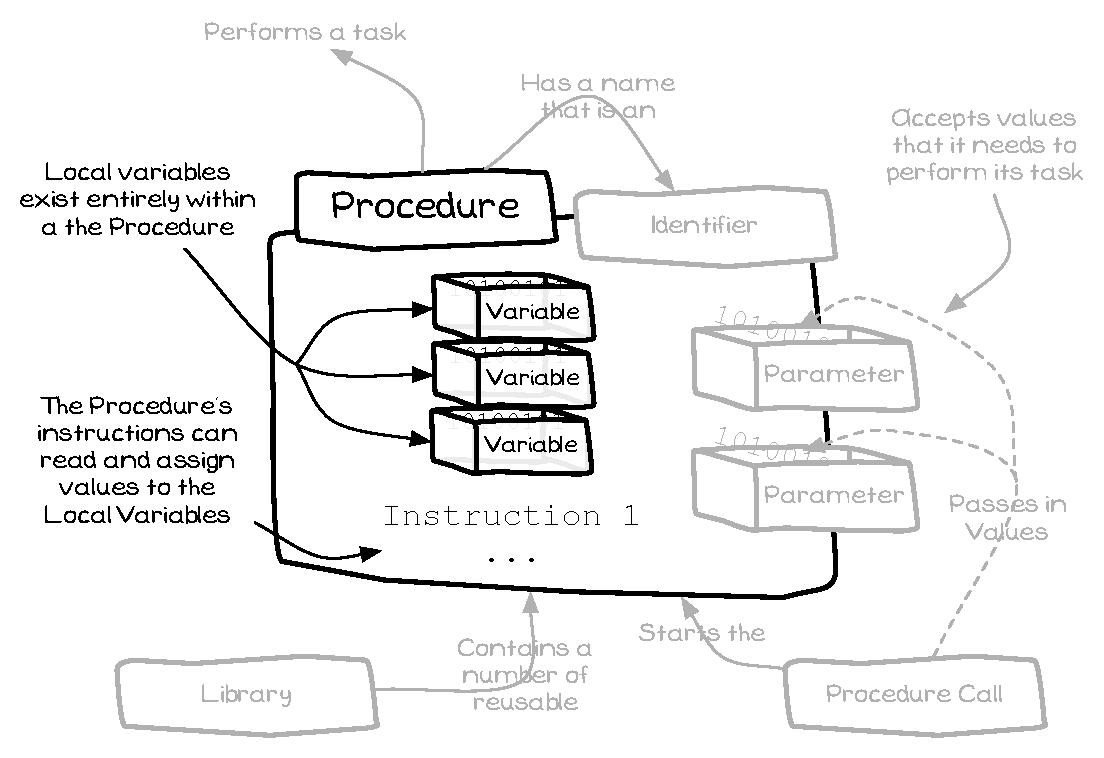
\includegraphics[width=\textwidth]{./topics/storing-using-data/diagrams/LocalVariables} 
   \caption{Variables declared within a Procedure are Local Variables}
   \label{fig:storing-using-data-local-variables}
\end{figure}

\mynote{
\begin{itemize}
  \item Local Variable is the \textbf{term} given to a Variable that is declared within a Procedure.
  \item Variables that are declared within Procedures are called \textbf{Local Variables}.
  \item Local Variables are located \textbf{within} the Procedure they are declared in. 
  \item They can only be accessed by instructions in the Procedure.
  \item It is \textbf{good practice} to use Local Variables to store values. These variables can only be accessed from the instructions within the Procedure, this makes it easier to understand how the variable is being used and where it is being changed. 
  \item Space is allocated for the Local Variables when the Procedure is called.
  \item When the call ends, the Local Variables for that call are destroyed.
\end{itemize}
}

% subsection local_variable (end)